The following notes are from \href{https://www.isbns.fm/isbn/9780495110811/}{\textbi{Mathematical Statistics with Applications, 7\textsuperscript{th} ed.} by Wackerly, Mendenhall \& Scheaffer}.

\section{What Is Statistics?}

\subsection{Introduction}

\begin{defn}[\idx{statistics}]
    \textbi{Statistics} is a theory of information with inference-making as its objective.
\end{defn}

\begin{rmrk}[\idx{The objective of statistics}]
    The objective of statistics is to make an inference about a population based on information contained in a sample from that population and to provide an associated measure of goodness for the inference.
\end{rmrk}

\begin{defn}[\idx{population}]
    A \textbi{population} is the large body of data that is the target of our interest.
\end{defn}

\begin{defn}[\idx{sample}]
    A \textbi{sample} is a subset selected from a population.
\end{defn}

\subsection{Characterizing a Set of Measurements: Graphical Methods}

\begin{note}[\idx{relative frequency histogram}]
    Given data set $[2.1,2.4,2.2,2.3,2.7,2.5,2.4,2.6.2.6,2.9]$ we can construct the \textbi{relative frequency histogram}:

    \begin{figure}[h]
        \vspace{-10pt}
        \centering
        % Created by tikzDevice version 0.12.6 on 2023-12-15 12:40:39
% !TEX encoding = UTF-8 Unicode
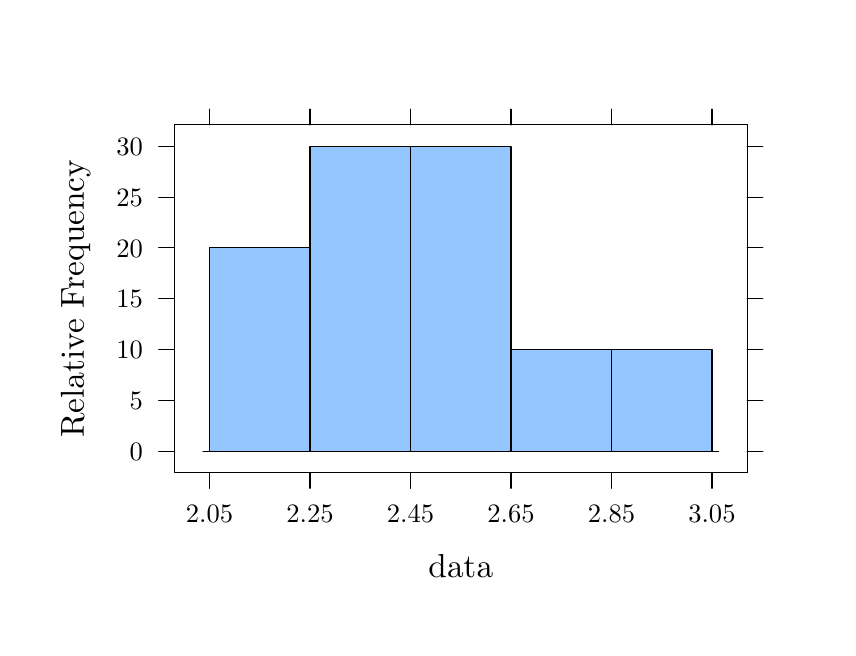
\begin{tikzpicture}[x=1pt,y=1pt]
\definecolor{fillColor}{RGB}{255,255,255}
\path[use as bounding box,fill=fillColor,fill opacity=0.00] (0,0) rectangle (289.08,216.81);
\begin{scope}
\path[clip] (  0.00,  0.00) rectangle (289.08,216.81);

\path[] (  0.00,  0.00) rectangle (289.08,216.81);
\definecolor{drawColor}{RGB}{0,0,0}

\node[text=drawColor,anchor=base,inner sep=0pt, outer sep=0pt, scale=  1.20] at (156.48, 18.07) {data};
\end{scope}
\begin{scope}
\path[clip] (  0.00,  0.00) rectangle (289.08,216.81);
\definecolor{drawColor}{RGB}{0,0,0}

\node[text=drawColor,rotate= 90.00,anchor=base,inner sep=0pt, outer sep=0pt, scale=  1.20] at ( 20.31,118.85) {Relative Frequency};
\end{scope}
\begin{scope}
\path[clip] (  0.00,  0.00) rectangle (289.08,216.81);
\definecolor{drawColor}{RGB}{0,0,0}

\path[draw=drawColor,line width= 0.4pt,line join=round,line cap=round] ( 65.71,181.67) -- ( 65.71,187.36);

\path[draw=drawColor,line width= 0.4pt,line join=round,line cap=round] (102.02,181.67) -- (102.02,187.36);

\path[draw=drawColor,line width= 0.4pt,line join=round,line cap=round] (138.33,181.67) -- (138.33,187.36);

\path[draw=drawColor,line width= 0.4pt,line join=round,line cap=round] (174.64,181.67) -- (174.64,187.36);

\path[draw=drawColor,line width= 0.4pt,line join=round,line cap=round] (210.95,181.67) -- (210.95,187.36);

\path[draw=drawColor,line width= 0.4pt,line join=round,line cap=round] (247.26,181.67) -- (247.26,187.36);
\end{scope}
\begin{scope}
\path[clip] (  0.00,  0.00) rectangle (289.08,216.81);
\definecolor{drawColor}{RGB}{0,0,0}

\path[draw=drawColor,line width= 0.4pt,line join=round,line cap=round] ( 53.00, 63.75) -- ( 47.31, 63.75);

\path[draw=drawColor,line width= 0.4pt,line join=round,line cap=round] ( 53.00, 82.12) -- ( 47.31, 82.12);

\path[draw=drawColor,line width= 0.4pt,line join=round,line cap=round] ( 53.00,100.49) -- ( 47.31,100.49);

\path[draw=drawColor,line width= 0.4pt,line join=round,line cap=round] ( 53.00,118.85) -- ( 47.31,118.85);

\path[draw=drawColor,line width= 0.4pt,line join=round,line cap=round] ( 53.00,137.22) -- ( 47.31,137.22);

\path[draw=drawColor,line width= 0.4pt,line join=round,line cap=round] ( 53.00,155.59) -- ( 47.31,155.59);

\path[draw=drawColor,line width= 0.4pt,line join=round,line cap=round] ( 53.00,173.96) -- ( 47.31,173.96);

\node[text=drawColor,anchor=base east,inner sep=0pt, outer sep=0pt, scale=  0.96] at ( 41.62, 60.45) {0};

\node[text=drawColor,anchor=base east,inner sep=0pt, outer sep=0pt, scale=  0.96] at ( 41.62, 78.81) {5};

\node[text=drawColor,anchor=base east,inner sep=0pt, outer sep=0pt, scale=  0.96] at ( 41.62, 97.18) {10};

\node[text=drawColor,anchor=base east,inner sep=0pt, outer sep=0pt, scale=  0.96] at ( 41.62,115.55) {15};

\node[text=drawColor,anchor=base east,inner sep=0pt, outer sep=0pt, scale=  0.96] at ( 41.62,133.92) {20};

\node[text=drawColor,anchor=base east,inner sep=0pt, outer sep=0pt, scale=  0.96] at ( 41.62,152.28) {25};

\node[text=drawColor,anchor=base east,inner sep=0pt, outer sep=0pt, scale=  0.96] at ( 41.62,170.65) {30};
\end{scope}
\begin{scope}
\path[clip] (  0.00,  0.00) rectangle (289.08,216.81);
\definecolor{drawColor}{RGB}{0,0,0}

\path[draw=drawColor,line width= 0.4pt,line join=round,line cap=round] ( 65.71, 56.04) -- ( 65.71, 50.35);

\path[draw=drawColor,line width= 0.4pt,line join=round,line cap=round] (102.02, 56.04) -- (102.02, 50.35);

\path[draw=drawColor,line width= 0.4pt,line join=round,line cap=round] (138.33, 56.04) -- (138.33, 50.35);

\path[draw=drawColor,line width= 0.4pt,line join=round,line cap=round] (174.64, 56.04) -- (174.64, 50.35);

\path[draw=drawColor,line width= 0.4pt,line join=round,line cap=round] (210.95, 56.04) -- (210.95, 50.35);

\path[draw=drawColor,line width= 0.4pt,line join=round,line cap=round] (247.26, 56.04) -- (247.26, 50.35);

\node[text=drawColor,anchor=base,inner sep=0pt, outer sep=0pt, scale=  0.96] at ( 65.71, 38.05) {2.05};

\node[text=drawColor,anchor=base,inner sep=0pt, outer sep=0pt, scale=  0.96] at (102.02, 38.05) {2.25};

\node[text=drawColor,anchor=base,inner sep=0pt, outer sep=0pt, scale=  0.96] at (138.33, 38.05) {2.45};

\node[text=drawColor,anchor=base,inner sep=0pt, outer sep=0pt, scale=  0.96] at (174.64, 38.05) {2.65};

\node[text=drawColor,anchor=base,inner sep=0pt, outer sep=0pt, scale=  0.96] at (210.95, 38.05) {2.85};

\node[text=drawColor,anchor=base,inner sep=0pt, outer sep=0pt, scale=  0.96] at (247.26, 38.05) {3.05};

\path[draw=drawColor,line width= 0.4pt,line join=round,line cap=round] (259.96, 63.75) -- (265.65, 63.75);

\path[draw=drawColor,line width= 0.4pt,line join=round,line cap=round] (259.96, 82.12) -- (265.65, 82.12);

\path[draw=drawColor,line width= 0.4pt,line join=round,line cap=round] (259.96,100.49) -- (265.65,100.49);

\path[draw=drawColor,line width= 0.4pt,line join=round,line cap=round] (259.96,118.85) -- (265.65,118.85);

\path[draw=drawColor,line width= 0.4pt,line join=round,line cap=round] (259.96,137.22) -- (265.65,137.22);

\path[draw=drawColor,line width= 0.4pt,line join=round,line cap=round] (259.96,155.59) -- (265.65,155.59);

\path[draw=drawColor,line width= 0.4pt,line join=round,line cap=round] (259.96,173.96) -- (265.65,173.96);
\end{scope}
\begin{scope}
\path[clip] ( 53.00, 56.04) rectangle (259.96,181.67);
\definecolor{drawColor}{RGB}{0,0,0}

\path[draw=drawColor,line width= 0.4pt,line join=round,line cap=round] ( 63.35, 63.75) --
	(249.62, 63.75);
\definecolor{fillColor}{RGB}{148,198,255}

\path[draw=drawColor,line width= 0.4pt,line join=round,line cap=round,fill=fillColor] ( 65.71, 63.75) rectangle (102.02,137.22);

\path[draw=drawColor,line width= 0.4pt,line join=round,line cap=round,fill=fillColor] (102.02, 63.75) rectangle (138.33,173.96);

\path[draw=drawColor,line width= 0.4pt,line join=round,line cap=round,fill=fillColor] (138.33, 63.75) rectangle (174.64,173.96);

\path[draw=drawColor,line width= 0.4pt,line join=round,line cap=round,fill=fillColor] (174.64, 63.75) rectangle (210.95,100.49);

\path[draw=drawColor,line width= 0.4pt,line join=round,line cap=round,fill=fillColor] (210.95, 63.75) rectangle (247.26,100.49);
\end{scope}
\begin{scope}
\path[clip] (  0.00,  0.00) rectangle (289.08,216.81);
\definecolor{drawColor}{RGB}{0,0,0}

\path[draw=drawColor,line width= 0.4pt,line join=round,line cap=round] ( 53.00, 56.04) rectangle (259.96,181.67);
\end{scope}
\end{tikzpicture}

        \vspace{-20pt}
        \caption{Relative Frequency Histogram}
        \label{fig:rfh}
    \end{figure}
    
    \begin{itemize}
        \item $2$ out of the $10$ values, $[2.1, 2.2]$, lie between $2.05$ and $2.25$.
        \item $3$ out of the $10$ values, $[2.4, 2.3, 2.4]$, lie between $2.25$ and $2.45$.
        \item $3$ out of the $10$ values, $[2.5, 2.6, 2.6]$, lie between $2.45$ and $2.65$.
        \item $1$ out of the $10$ values, $[2.7]$, lies between $2.65$ and $2.85$.
        \item $1$ out of the $10$ values, $[2.9]$, lies between $2.85$ and $3.05$.
    \end{itemize}
\end{note}

\begin{rmrk}
    When choosing the intervals of a histogram:
    \begin{enumerate}
        \item Choose so that it is impossible for a measurement to fall on a point of division. The idea is to separate the data into distinct buckets and look at what perecentage of the total data set is contained in each bucket. The `buckets' correspond to the chosen intervals. If intervals are chosen such that a data point falls exactly between two intervals, then it's ambiguous as to which interval the data point lies in.
        \item You could choose an interval that contains every data point but this defeats the purpose of using the histogram to visualize the relative frequency of data in the data set. You could also choose many small intervals which each contain at most one data point but this would defeat the purpose of broadly visualizing the relative frequency of data in the data set. The number of intervals should scale appropriately with the size of the data set.
    \end{enumerate}
\end{rmrk}

\begin{note}
    The probability that an arbitrary value from a data set will lie in a given interval of a relative frequency histogram for that data set is equal to the percentage of the total area of the histogram lying over that interval.
\end{note}

\begin{exmp}
    The total area of the histogram of Fig.\ref{fig:rfh} is: $$(2.25 - 2.05)\cdot 0.2 + (2.45 - 2.05)\cdot 0.3 + (2.65 - 2.45)\cdot 0.3 + (2.85 - 2.65)\cdot 0.1 + (3.05 - 2.85)\cdot 0.1 = 0.2$$
    The area of the histogram in the interval $[2.05, 2.45]$ is: $$(2.25 - 2.05)\cdot 0.2 + (2.45 - 2.05)\cdot 0.3 = 0.1$$
    So, based on this histogram, the probability that an arbitrary data point lies between $2.05$ and $2.45$ is: $$0.1 / 0.2 = 0.5 = 50\%$$
\end{exmp}

\subsection{Characterizing a Set of Measurements: Numerical Methods}

\begin{defn}[\idx{mean}]
    Given a data set $[y_{1}, y_{2}, \ldots, y_{n}]$, the \textbi{mean} of the data set is given by: $$\mu = \bar{y} = \frac{1}{n} \sum_{i=1}^{n} y_{i}$$
\end{defn}

\begin{nota}[\idx{mean}: \idx{$\mu$}, \idx{$\bar{y}$}]
    $\mu$ for population, $\bar{y}$ for sample. $\bar{y}$ is read ``$y$ bar''.
\end{nota}

\begin{defn}[\idx{population variance}]
    Given a population $[y_{1}, y_{2}, \ldots, y_{n}]$, the \textbi{population variance} of the population is given by: $$\sigma^{2} = \frac{1}{n} \sum_{i=1}^{n} (y_{i} - \mu)^{2}$$
\end{defn}

\begin{nota}[\idx{population variance}: \idx{$\sigma^{2}$}]
\end{nota}

\pagebreak
\begin{defn}[\idx{sample variance}]
    Given a sample $[y_{1}, y_{2}, \ldots, y_{n}]$, the \textbi{sample variance} of the population is given by: $$s^{2} = \frac{1}{n-1} \sum_{i=1}^{n} (y_{i} - \bar{y})^{2}$$
\end{defn}

\begin{rmrk}
    It isn't immediately obvious why the denominator of the sample variance should be $n-1$ instead of $n$ like in the popluation variance. The reason for this will be explained later after developing some concepts.
\end{rmrk}

\begin{nota}[\idx{sample variance}: \idx{$s^{2}$}]
\end{nota}

\begin{defn}[\idx{standard deviation}]
    \begin{itemize}
        \item Given a population, a \textbi{standard deviation} of the population is given by $\sigma = \sqrt{\sigma^{2}}$ where $\sigma^{2}$ is the population variance.
        \item Given a sample, the \textbi{standard deviation} of the sample is given by $s = \sqrt{s^{2}}$ where $s^{2}$ is the sample variance.
    \end{itemize}
\end{defn}

\begin{nota}[\idx{standard deviation}: \idx{$\sigma$}, \idx{s}]
    $\sigma$ for population, $s$ for sample.
\end{nota}

\begin{note}[\idx{Empirical Rule}]
    For a distribution of measurements that is approximately normal (bell-shaped):
    \begin{itemize}
        \item the interval $\mu \pm \sigma$ contains approx. $68\%$ of measurements
        \item the interval $\mu \pm 2\sigma$ contains approx. $95\%$ of measurements
        \item the interval $\mu \pm 3\sigma$ contains approx. almost all measurements
    \end{itemize}

    \begin{figure}[h]
        \vspace{-40pt}
        \centering
        % Created by tikzDevice version 0.12.6 on 2023-12-16 17:47:11
% !TEX encoding = UTF-8 Unicode
\begin{tikzpicture}[x=1pt,y=1pt]
\definecolor{fillColor}{RGB}{255,255,255}
\path[use as bounding box,fill=fillColor,fill opacity=0.00] (0,0) rectangle (433.62,216.81);
\begin{scope}
\path[clip] ( 49.20, 61.20) rectangle (408.42,167.61);
\definecolor{drawColor}{RGB}{0,0,0}

\path[draw=drawColor,line width= 0.4pt,line join=round,line cap=round] ( 62.50, 65.14) --
	( 65.83, 65.20) --
	( 69.16, 65.27) --
	( 72.48, 65.37) --
	( 75.81, 65.48) --
	( 79.14, 65.62) --
	( 82.46, 65.79) --
	( 85.79, 65.99) --
	( 89.11, 66.24) --
	( 92.44, 66.53) --
	( 95.77, 66.88) --
	( 99.09, 67.30) --
	(102.42, 67.80) --
	(105.74, 68.38) --
	(109.07, 69.05) --
	(112.40, 69.84) --
	(115.72, 70.74) --
	(119.05, 71.78) --
	(122.37, 72.96) --
	(125.70, 74.30) --
	(129.03, 75.81) --
	(132.35, 77.50) --
	(135.68, 79.39) --
	(139.00, 81.48) --
	(142.33, 83.77) --
	(145.66, 86.28) --
	(148.98, 89.00) --
	(152.31, 91.94) --
	(155.64, 95.09) --
	(158.96, 98.44) --
	(162.29,101.98) --
	(165.61,105.70) --
	(168.94,109.57) --
	(172.27,113.57) --
	(175.59,117.66) --
	(178.92,121.82) --
	(182.24,126.01) --
	(185.57,130.19) --
	(188.90,134.31) --
	(192.22,138.34) --
	(195.55,142.21) --
	(198.88,145.90) --
	(202.20,149.34) --
	(205.53,152.50) --
	(208.85,155.33) --
	(212.18,157.80) --
	(215.51,159.87) --
	(218.83,161.52) --
	(222.16,162.71) --
	(225.48,163.43) --
	(228.81,163.67) --
	(232.14,163.43) --
	(235.46,162.71) --
	(238.79,161.52) --
	(242.11,159.87) --
	(245.44,157.80) --
	(248.77,155.33) --
	(252.09,152.50) --
	(255.42,149.34) --
	(258.75,145.90) --
	(262.07,142.21) --
	(265.40,138.34) --
	(268.72,134.31) --
	(272.05,130.19) --
	(275.38,126.01) --
	(278.70,121.82) --
	(282.03,117.66) --
	(285.35,113.57) --
	(288.68,109.57) --
	(292.01,105.70) --
	(295.33,101.98) --
	(298.66, 98.44) --
	(301.98, 95.09) --
	(305.31, 91.94) --
	(308.64, 89.00) --
	(311.96, 86.28) --
	(315.29, 83.77) --
	(318.61, 81.48) --
	(321.94, 79.39) --
	(325.27, 77.50) --
	(328.59, 75.81) --
	(331.92, 74.30) --
	(335.25, 72.96) --
	(338.57, 71.78) --
	(341.90, 70.74) --
	(345.22, 69.84) --
	(348.55, 69.05) --
	(351.88, 68.38) --
	(355.20, 67.80) --
	(358.53, 67.30) --
	(361.85, 66.88) --
	(365.18, 66.53) --
	(368.51, 66.24) --
	(371.83, 65.99) --
	(375.16, 65.79) --
	(378.48, 65.62) --
	(381.81, 65.48) --
	(385.14, 65.37) --
	(388.46, 65.27) --
	(391.79, 65.20) --
	(395.12, 65.14);
\end{scope}
\begin{scope}
\path[clip] ( 49.20, 61.20) rectangle (408.42,167.61);
\definecolor{drawColor}{RGB}{0,0,0}

\path[draw=drawColor,line width= 0.4pt,line join=round,line cap=round] ( 86.26, 64.93) -- ( 86.26, 66.02);

\path[draw=drawColor,line width= 0.4pt,line join=round,line cap=round] (133.78, 64.93) -- (133.78, 78.29);

\path[draw=drawColor,line width= 0.4pt,line join=round,line cap=round] (181.29, 64.93) -- (181.29,124.82);

\path[draw=drawColor,line width= 0.4pt,line join=round,line cap=round] (228.81, 64.93) -- (228.81,163.67);

\path[draw=drawColor,line width= 0.4pt,line join=round,line cap=round] (276.33, 64.93) -- (276.33,124.82);

\path[draw=drawColor,line width= 0.4pt,line join=round,line cap=round] (323.84, 64.93) -- (323.84, 78.29);

\path[draw=drawColor,line width= 0.4pt,line join=round,line cap=round] (371.36, 64.93) -- (371.36, 66.02);
\end{scope}
\begin{scope}
\path[clip] (  0.00,  0.00) rectangle (433.62,216.81);
\definecolor{drawColor}{RGB}{0,0,0}

\path[draw=drawColor,line width= 0.4pt,line join=round,line cap=round] ( 86.26, 64.93) -- (371.36, 64.93);

\path[draw=drawColor,line width= 0.4pt,line join=round,line cap=round] ( 86.26, 64.93) -- ( 86.26, 58.93);

\path[draw=drawColor,line width= 0.4pt,line join=round,line cap=round] (133.78, 64.93) -- (133.78, 58.93);

\path[draw=drawColor,line width= 0.4pt,line join=round,line cap=round] (181.29, 64.93) -- (181.29, 58.93);

\path[draw=drawColor,line width= 0.4pt,line join=round,line cap=round] (228.81, 64.93) -- (228.81, 58.93);

\path[draw=drawColor,line width= 0.4pt,line join=round,line cap=round] (276.33, 64.93) -- (276.33, 58.93);

\path[draw=drawColor,line width= 0.4pt,line join=round,line cap=round] (323.84, 64.93) -- (323.84, 58.93);

\path[draw=drawColor,line width= 0.4pt,line join=round,line cap=round] (371.36, 64.93) -- (371.36, 58.93);

\node[text=drawColor,anchor=base,inner sep=0pt, outer sep=0pt, scale=  1.00] at ( 86.26, 43.33) {$\mu - 3\sigma$};

\node[text=drawColor,anchor=base,inner sep=0pt, outer sep=0pt, scale=  1.00] at (133.78, 43.33) {$\mu - 2\sigma$};

\node[text=drawColor,anchor=base,inner sep=0pt, outer sep=0pt, scale=  1.00] at (181.29, 43.33) {$\mu - \sigma$};

\node[text=drawColor,anchor=base,inner sep=0pt, outer sep=0pt, scale=  1.00] at (228.81, 43.33) {$\mu$};

\node[text=drawColor,anchor=base,inner sep=0pt, outer sep=0pt, scale=  1.00] at (276.33, 43.33) {$\mu + \sigma$};

\node[text=drawColor,anchor=base,inner sep=0pt, outer sep=0pt, scale=  1.00] at (323.84, 43.33) {$\mu + 2\sigma$};

\node[text=drawColor,anchor=base,inner sep=0pt, outer sep=0pt, scale=  1.00] at (371.36, 43.33) {$\mu + 3\sigma$};
\end{scope}
\end{tikzpicture}

        \vspace{-40pt}
        \caption{Empirical Rule}
        \label{fig:emprule}
    \end{figure}
\end{note}

\begin{lemm}
    $$s^{2} = \frac{1}{n-1} \sum_{i=1}^{n} (y_{i} - \bar{y})^{2} = \frac{1}{n-1} \left[\sum_{i=1}^{n} y_{i}^{2} - \frac{1}{n} \left(\sum_{i=1}^{n} y_{i}\right)^{2}\right]$$
\end{lemm}

\begin{proof}
    \begin{align*}
        s^{2} &= \frac{1}{n-1} \sum_{i=1}^{n} (y_{i} - \bar{y})^{2}\\
              &= \frac{1}{n-1} \sum_{i=1}^{n} (y_{i}^{2} -2\bar{y} y_{i} + \bar{y}^{2})\\
              &= \frac{1}{n-1} \left[\sum_{i=1}^{n} y_{i}^{2} -2\bar{y} \sum_{i=1}^{n} y_{i} + \sum_{i=1}^{n} \bar{y}^{2}\right]\\
              &= \frac{1}{n-1} \left[\sum_{i=1}^{n} y_{i}^{2} -2n\bar{y}^{2} + n\bar{y}^{2}\right]\\
              &= \frac{1}{n-1} \left[\sum_{i=1}^{n} y_{i}^{2} -n\bar{y}^{2}\right]\\
              &= \frac{1}{n-1} \left[\sum_{i=1}^{n} y_{i}^{2} -n\left(\frac{1}{n} \sum_{i=1}^{n} y_{i}\right)^{2}\right]\\
              &= \frac{1}{n-1} \left[\sum_{i=1}^{n} y_{i}^{2} -\frac{1}{n}\left(\sum_{i=1}^{n} y_{i}\right)^{2}\right]\\    
    \end{align*}
\end{proof}

\begin{defn}[\idx{range}]
    Given a data set, the \textbi{range} of the data set is the difference between the largest and smallest values of the data set. 
\end{defn}

\begin{note}[\idx{Quarter Range Rule}]
    Since $\sim 95\%$ -- i.e. most -- of all normally-distributed measurements lie within two standard deviations from the mean, standard deviation can be estimated as \nicefrac{1}{4} the range of the measurements.
\end{note}

\subsubsection{Exercises}

